% \RequirePackage{plautopatch} % If use uplatex, enable this line.
\documentclass[twocolumn,paper=a4paper,landscape,fontsize=9pt]{jlreq}
\usepackage{url}
\usepackage{graphicx}
\usepackage{amsmath}
\usepackage{here}

\usepackage[backend=bibtex,sorting=none]{biblatex}
\usepackage{ipsj-tohoku}

\bibliography{cites}

\title{タンパク質配列グラフ表示画像の作成に適したアミノ酸指標の組み合わせの探索}

\author{土山啓汰\thanks{1} 水田智史\thanks{1}}

% \TechrepVolNoDate{2021-6}{}{2022/02/21}
% \Copyright{Information Processing Society of Japan}

\begin{document}

\affiliation{1}{情報処理学会東北支部大学}

\maketitle

\begin{abstract}
 本研究ではアライメントに依らないタンパク質アミノ酸配列比較の手法を検討する。まず、アミノ酸にAAindexのアミノ酸指標を用いて三次元座標群を作成する。それに対して主成分分析を行い、得られた第一主成分、及び第二主成分を利用してコサイン類似度やスペクトル解析を適用して距離行列とする。距離行列から系統樹を生成し、マルチプルアライメントにより得られる系統樹とunweighted robinson-foulds距離により結果を比較する。
\end{abstract}

\section{イントロダクション}
\subsection{研究の背景と目的}
本研究ではタンパク質のアミノ酸配列を扱う。アミノ酸はタンパク質の構成要素である。20種類の異なるアミノ酸がタンパク質の合成に用いられる。各タンパク質の形状や他の特性はそこに含まれるアミノ酸の配列の仕方によって決定し、アミノ酸配列が似ているほど機能や性質が類似している可能性が高いと言える。 \\
 タンパク質のアミノ酸配列間の類似性を評価する方法として、一般的にアライメントが用いられている。しかし、配列長が$N$と$N$の場合は動的計画法により$O(N^2)$の時間計算量となり、肥大な計算時間が必要となる。そのため、本研究室ではアライメントに依らないタンパク質アミノ酸配列比較の手法として、アミノ酸に何らかの2次元ベクトルを割り当てグラフィカル表現を行うことが提案されてきた。これにより、グラフが似ていれば類似性が高いといったような直観的な評価が可能となる。また、同時に定量的な評価も行う。\\
 本研究では、この手法の精度を高めるために、アミノ酸のベクトルの割り当て方に注目し、遺伝子解析同等の系統樹を早く作成することを目的としている。


\section{方法}
\subsection{ベクトルの割り当て}
タンパク質のアミノ酸配列を3次元座標群化するためにアミノ酸20種にベクトルを割り当てる。本研究では、AAindexに掲載されているアミノ酸指標566種類のうち、指標内に重複した値が使用されている、外れ値が含まれる、もしくは指標間で直交している指標を除外した114種類のアミノ酸指標を使用する。\\
 具体的には、114種類のうち3種類のアミノ酸指標を選択し、そのアミノ酸指標間の相関係数の絶対値の和を利用してベクトルを割り当てる。本研究では、絶対値の和を昇順に並べた上位1000位までの指標を研究対象とし、選択したアミノ酸指標3種類をそれぞれ$x$, $y$, $z$座標に割り当てた。

\subsection{三次元座標群の作成}
アミノ酸に割り当てたベクトルを元に三次元座標群を作成する。例として配列ACDEFに対する座標群を表に示す。

\newpage
\begin{table}[h]
\centering
\caption{3次元座標群の例}
\scalebox{1}[1]{
\begin{tabular}{c|lll}\hline
&X&Y&Z \\ \hline
&0&0&0 \\[-2mm]
A&&↓&\\[-2mm]
&0&0.83&1.083\\[-2mm]
C&&↓&\\[-2mm]
&1.007&-0.177&2.942\\[-2mm]
D&&↓&\\[-2mm]
&1.629&0.9&4.205\\[-2mm]
E&&↓&\\[-2mm]
&2.205&-0.1&5.377\\[-2mm]
F&&↓&\\[-2mm]
&1.51&-1.305&6.79\\ \hline
\end{tabular}}
\end{table}

また、図にグラフ化した3次元座標群の例(ヒトとゴリラのND5配列グラフ、ヒトとドブネズミの配列グラフ)を示す。近縁種同士のグラフの概形が似ていることが直観的にわかる。

\begin{figure}[H]
  \centering
  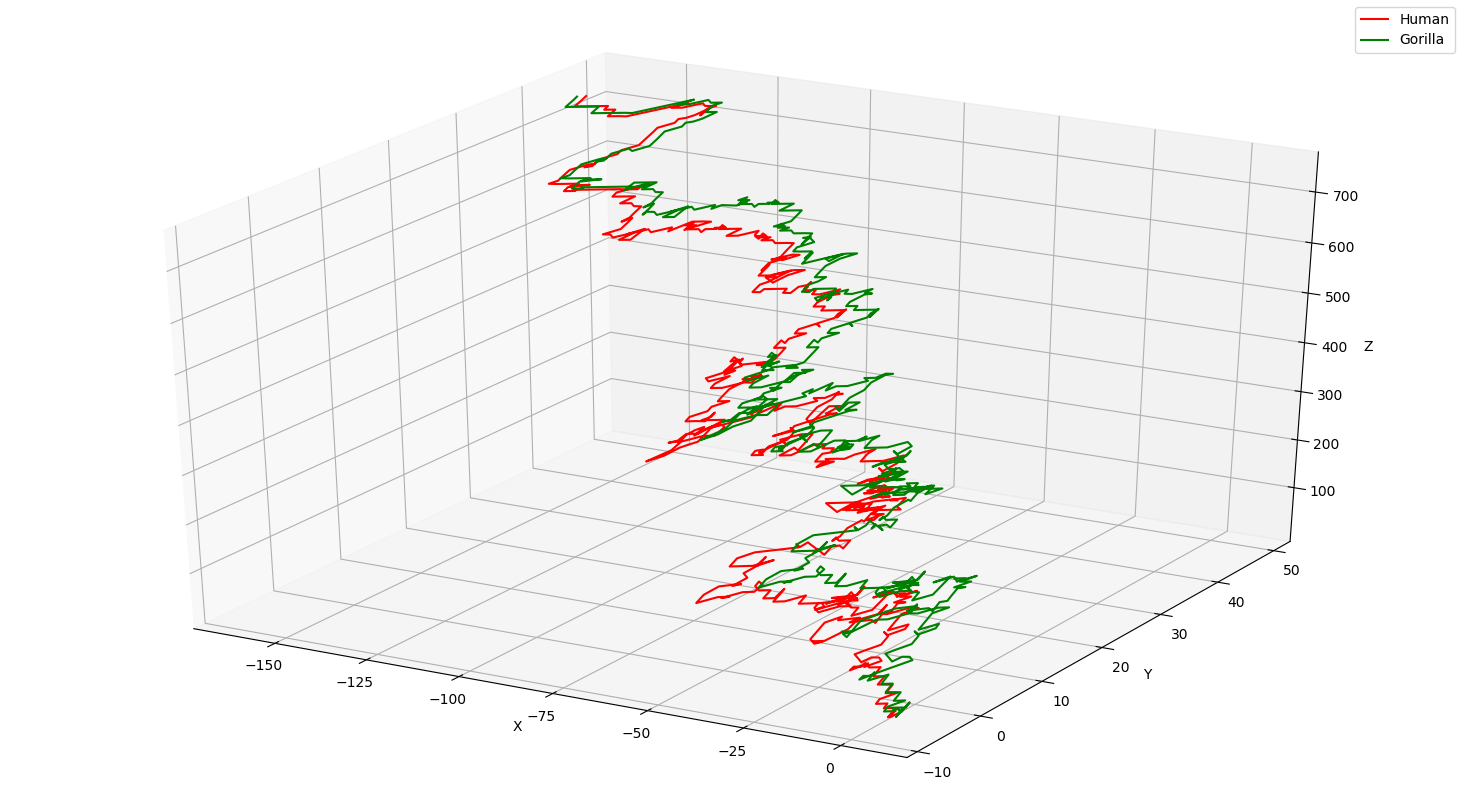
\includegraphics[width=70mm]{human_gorilla.png}
  \caption{ヒトとゴリラのND5配列グラフ}
\end{figure}

\begin{figure}[H]
  \centering
  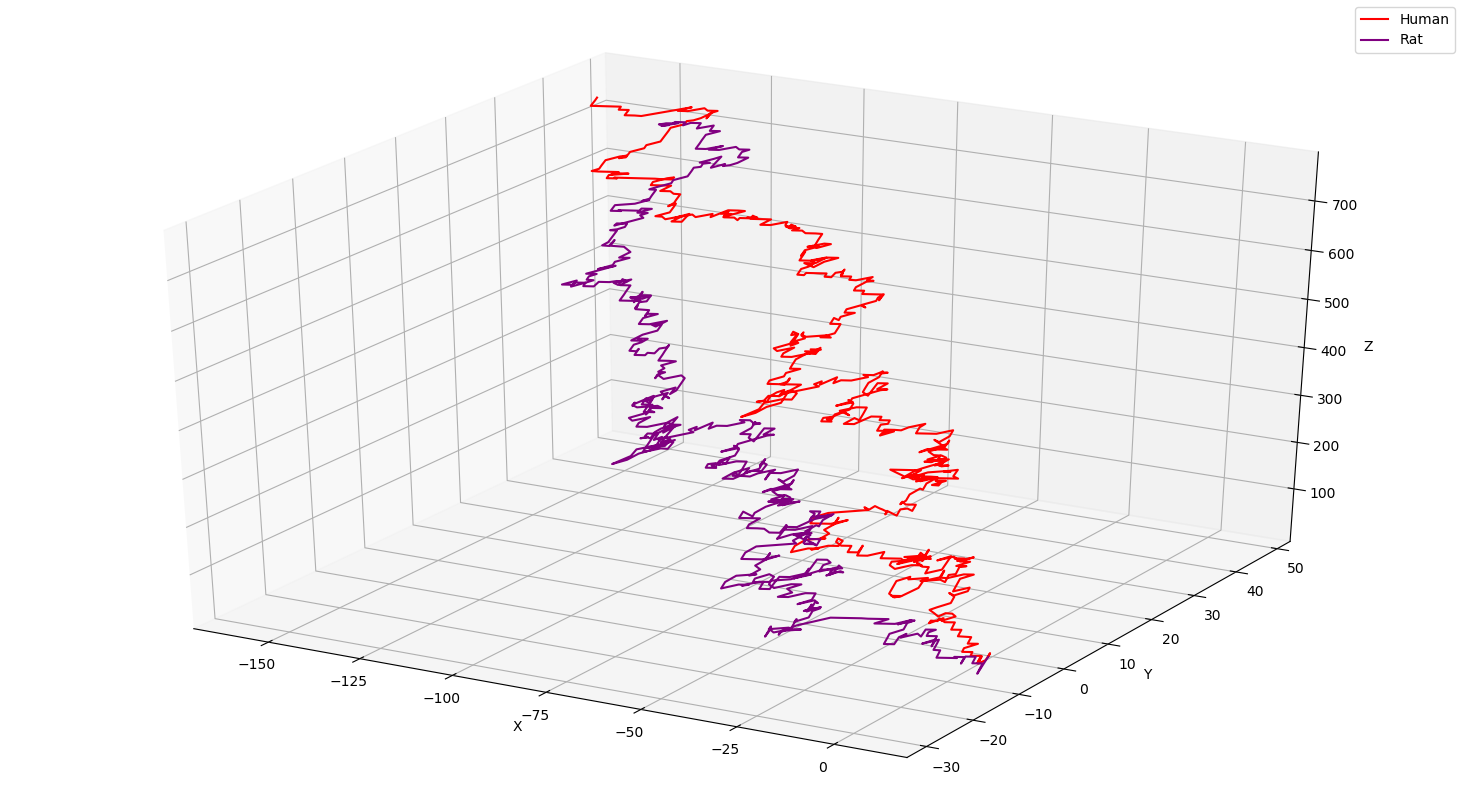
\includegraphics[width=70mm]{human_rat.png}
  \caption{ヒトとドブネズミのND5配列グラフ}
\end{figure}
  

\subsection{重み}
アミノ酸にベクトルを与えた後、配列の情報をより反映させるために重み利用する。重みは自己情報量を用いて
\begin{equation}
-\log10 \frac{各アミノ酸の数}{アミノ酸の総数} \\
\end{equation}

により求めた。この重みをそれぞれのベクトルに掛けたものを本研究では使用する。

\begin{table}[h]
\centering
\caption{重み}
\scalebox{1}[1]{
\begin{tabular}{|cc|cc|cc|} \hline
アミノ酸 & 重み & アミノ酸 & 重み & アミノ酸 & 重み\\ \hline
A &1.083 &I &1.228 &R &1.257 \\[-2mm]
C &1.859 &K &1.236 &S &1.178 \\[-2mm]
D &1.263 &L &1.015 &T &1.271 \\[-2mm]
E &1.172 &M &1.617 &V &1.163 \\[-2mm]
F &1.413 &N &1.391 &W &1.959 \\[-2mm]
G &1.150 &P &1.324 &Y &1.535 \\[-2mm]
H &1.643 &Q &1.405 &\ &\ \\ \hline
\end{tabular}
}
\end{table}

\subsection{距離行列の求め方}
生物の配列のグラフ化行った後、それぞれのグラフに対して主成分分析を行う。本研究では、求めた主成分に対してコサイン類似度を適用した距離行列、スペクトル解析を行った後、コサイン類似度を適用した距離行列(以下スペクトル解析)をそれぞれ求めた。

\subsubsection{主成分分析}
生物の配列に対して主成分分析を行う。主成分は、第一主成分の分散を最大化し、続く主成分はそれまでに決定した主成分と直交するという拘束条件の下で分散を最大化するようにして選ばれる。
% 主成分の分散を最大化することは、観測値の変化に対する説明能力を可能な限り主成分に持たせる目的で行われる。
第一主成分は生物種同士の三次元座標群から計算した分散共分散行列の固有値問題を解いたときの最大固有値に属する固有ベクトルである。本研究の生物の配列は三次元座標群であるため、以下の分散共分散行列$\hat{I}$を解けばよい。ここで、$S_{xx}$は$x$の分散であり、$S_{xy}$は$x$と$y$の共分散である。

\begin{equation}
  \hat{I}=
\begin{pmatrix}
  S_{xx} & S_{xy} & S_{xz} \\
  S_{yx} & S_{yy} & S_{yz} \\
  S_{zx} & S_{zy} & S_{zz}
\end{pmatrix}
\end{equation}

\subsubsection{コサイン類似度}
主成分分析で求めたそれぞれの第一主成分のなす角を$θ$として$cosθ$を計算する。方向ベクトルを$\vec{a}$、$\vec{b}$とすると、$cosθ$は以下の式で求められる。

\begin{equation}
\cos = \frac{\vec{a}\cdot\vec{b}}{|\vec{a}||\vec{b}|}
\end{equation}

上記の式の値をアークコサインを用いて求めた$θ$の値を距離と定義した。

\subsubsection{スペクトル解析}
生物の配列の位置を$x$軸、主成分分析で求めた第二主成分を$y$軸とした二次元グラフについて、離散フーリエ変換を用いて周波数成分を抽出する。
\begin{equation}
F(t) =\sum^{N-1}_{x = 0}f(x)\exp(\frac{-i2\pi tx}{N})
\end{equation}

抽出した周波数成分のパワースペクトルを求める。
\begin{equation}
powerspectre = \sqrt[]{real^2+imag^2}
\end{equation}

パワースペクトルのコサイン類似度を求めた後、アークコサインを用いて求めた$θ$の値を距離と定義した。

\section{結果}
\subsection{実験に用いたデータ}
本研究で使用した生物種は以前の研究[1]と同じ哺乳類の9種類で、以下の表の通りである。ミトゴンドリアDNAにコードされているNDAHデヒドロゲナーゼサブユニット5(以下ND5タンパク質)を使用した。

\begin{table}[h]
\centering
\caption{使用した生物種}
\scalebox{1}[1]{
\begin{tabular}{|l|c|c|} \hline
英名(和名)& accession no. & 配列長 \\ \hline
Human:ヒト & AP\_000649 & 603 \\[-2mm]
Gorilla:ゴリラ & NP\_008222 & 603 \\[-2mm]
Pygmy chimpanzee(P.chi.):ボノボ & NP\_008209 & 603 \\[-2mm]
Common chimpanzee(C.chi.):チンパンジー & NP\_008196 & 603 \\[-2mm]
Fin whale(F.wh.):ナガスクジラ & NP\_006899 & 606 \\[-2mm]
Blue whale(B.wh.):シロナガスクジラ & NP\_007066 & 606 \\[-2mm]
Rat:ドブネズミ & AP\_004902 & 610 \\[-2mm]
Mouse:ハツカネズミ  & NP\_904338 & 607 \\[-2mm]
Opposum(Oposs.):オポッサム & NP\_007105 & 602 \\ \hline
\end{tabular}}
\end{table}

\subsection{距離行列}
表に距離行列の例を示す。選択したアミノ酸指標は、AAindexのアクセッション名JANJ780101、JUNJ780101、QIAN880107であり、これらは相関係数の絶対値の和が一番小さいものである。近縁種同士は距離が近く、遠縁種になるほど距離が距離が遠くなる。

\begin{table}[h]
  \centering
  \caption{距離行列}
  \scalebox{0.7}[0.7]{
  \begin{tabular}{|c|c|c|c|c|c|c|c|c|c|} \hline
   & Human & Gorilla & P.chi. & C.chi. & F.wh. & B.wh. & Rat & Mouse & Oposs. \\ \hline
  Human & 0.000000  & &  & & & & & &  \\ 
  Gorilla & 0.167204  & 0.000000  & & & & & & &  \\ 
  P.chi. & 0.160675  & 0.122393  & 0.000000  & &  & & & &  \\ 
  C.chi. & 0.090493  & 0.175291  & 0.140388  & 0.000000  & & & & &  \\
  F.wh. & 0.294511  & 0.276881  & 0.295638  & 0.271027  & 0.000000  & & & &  \\ 
  B.wh. & 0.278365  & 0.258424  & 0.280428  & 0.250166  & 0.084905  & 0.000000  & & &  \\ 
  Rat & 0.248776  & 0.220215  & 0.206657  & 0.221194  & 0.306087  & 0.274655  & 0.000000  & &  \\ 
  Mouse & 0.296341  & 0.397280  & 0.386362  & 0.309180  & 0.475488  & 0.457054  & 0.333129  & 0.000000  &  \\ 
  Oposs. & 0.326698  & 0.244100  & 0.220393  & 0.310439  & 0.347707  & 0.342740  & 0.227025  & 0.458697  & 0.000000  \\ \hline
  \end{tabular}}
  \end{table}

\subsection{系統樹の作成}
生物種に対して、Clustal Omegaを用いてマルチプルアライメントで作成した系統樹と、コサイン類似度、及びスペクトル解析で作成した系統樹をunweighted robinson-foulds距離(以下RF距離)で比較する。RF距離とは2つの系統樹を比べて樹形間距離を表す方法である。系統樹から内分枝をひとつ取り除くと2つの部分木ができるが、この部分木におけるOTU組成(OTU:近縁な個体をひとまとめに分類するための操作上の単位)を2つの系統樹で比べ、一致しなかった数を樹形間距離として表す。なお、系統樹の作成にはUPGMA法を用いる。\\
 以下に$x$軸に相関係数の絶対値の和を昇順に並べた際の順番を、$y$軸にマルチプルアライメントで作成した系統樹とのRF距離をとったグラフを示す。

\begin{figure}[H]
  \centering
  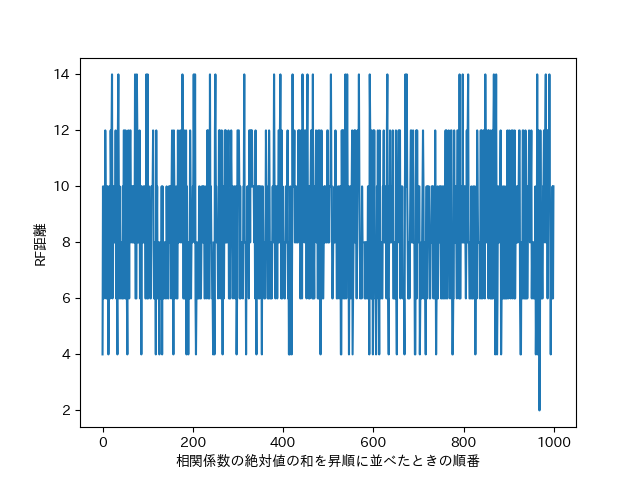
\includegraphics[width=70mm]{pca_treelist.png}
  \caption{マルチプルアライメントで作成した系統樹とコサイン類似度を利用して作成した系統樹のRF距離}
\end{figure}

\begin{figure}[H]
  \centering
  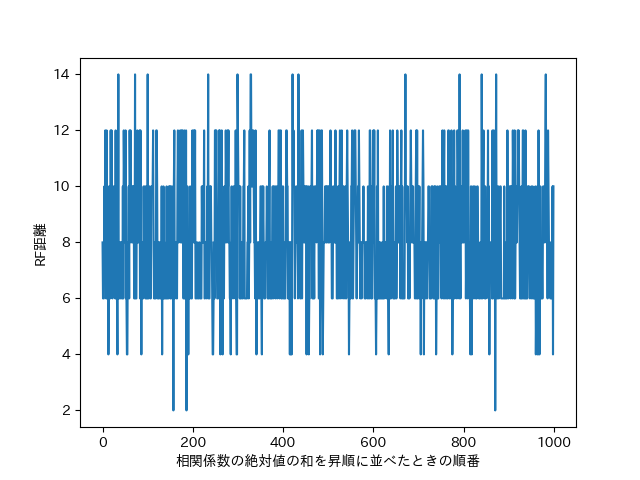
\includegraphics[width=70mm]{pca_treelist_o.png}
  \caption{マルチプルアライメントで作成した系統樹と、座標に重みをかけコサイン類似度を利用して作成した系統樹のRF距離}
\end{figure}

\begin{figure}[H]
  \centering
  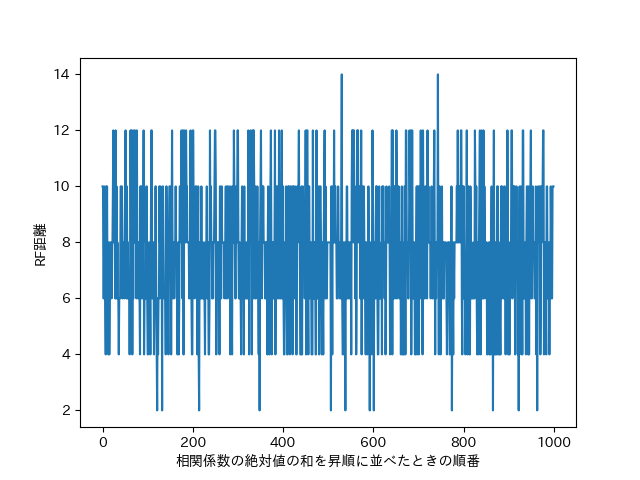
\includegraphics[width=70mm]{f_treelist.png}
  \caption{マルチプルアライメントで作成した系統樹とスペクトル解析を利用して作成した系統樹のRF距離}
\end{figure}

\begin{figure}[H]
  \centering
  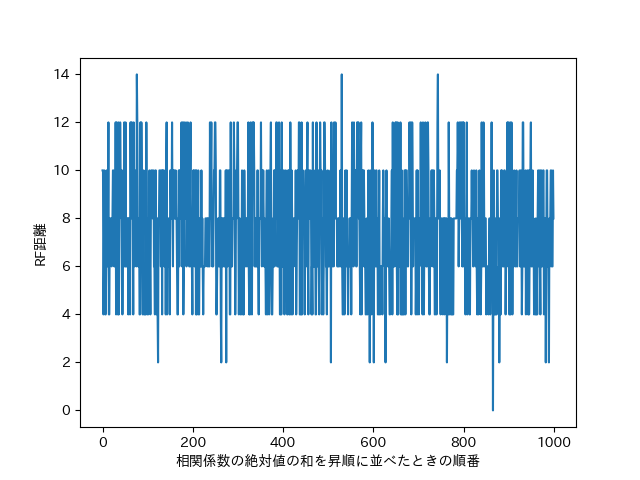
\includegraphics[width=70mm]{f_treelist_o.png}
  \caption{マルチプルアライメントで作成した系統樹と、座標に重みをかけスペクトル解析を利用して作成した系統樹のRF距離}
\end{figure}

マルチプルアライメントで得られた系統樹と同等の結果を示した($RF距離=0$)のは、AAindexのアミノ酸指標QIAN880138,RACS820102,HARY940101を使用し、座標に重みをかけ、スペクトル解析を利用して作成した系統樹であった。


\section{まとめと今後の課題}
 本研究では、タンパク質のアミノ酸配列を3次元グラフ化し、その第一主成分のなす角、及びスペクトル解析の結果から得られた周波数成分から距離を計算した。近縁種同士はグラフの概形が似ており、直観的に近縁種なのか遠縁種なのか判断でき、配列間を定量的に評価できた。\\
 本研究でマルチプルアライメントで得られた系統樹と同等の結果を示したアミノ酸指標について、大まかにQIAN880138はを表す。RACS820102は右巻きのα-helix領域における各アミノ酸の相対出現頻度を示す。HARY940101はタンパク質内部に埋もれた残基の平均体積を示す。これらが系統樹の作成に関与している可能性が示唆された。\\
 今後の課題として、より正確な系統樹を作成することが必要である。本研究で得られたRF距離は想定していたRF距離より大きく改善の余地がある。例えば、本研究では指標内に重複した値が使用されている、外れ値が含まれる、もしくは指標間で直交している指標を除外した114種類のアミノ酸指標を使用しているが、より適切な条件付けを行う方法を検討する。また、主成分分析、コサイン類似度及びスペクトル解析を行っているが、他の特徴量を使用することが挙げられる。

\begin{thebibliography}{9}
  \bibitem{agata} Agata,C ,Dorota,B ,Piotr,W and Tim,C "20D-dynamic representation of protein sequences" Ge-nomics Volume 107, Issue 1, January 2016, Pages 16-23
\end{thebibliography}

\end{document}
